
%%%%%%%%%%%%%%%%%%%%%%%%%%%%%%%%%%%%%%%%%%%%%%%%%%%%%%%%%%%%%%%%%%%%%%%%%%%%%%%%%%%%%%%%%%%%%%%%%%%%
%%%%%%%%%%%%%%%%%%%%%%%%%%%%%%%%%%%%%%%%%%%%%%%%%%%%%%%%%%%%%%%%%%%%%%%%%%%%%%%%%%%%%%%%%%%%%%%%%%%%
%%%%%%%%%%%%%%%%%%%%%%%%%%%%%%%%%%%%%%%%%%%%%%%%%%%%%%%%%%%%%%%%%%%%%%%%%%%%%%%%%%%%%%%%%%%%%%%%%%%%
%%%%%%%%%%%%%%%%%%%%%%%%%%%%%%%%%%%%%%%%%%%%%%%%%%%%%%%%%%%%%%%%%%%%%%%%%%%%%%%%%%%%%%%%%%%%%%%%%%%%
%%%%%%%%%%%%%%%%%%%%%%%%%%%%%%%%%%%%%%%%%%%%%%%%%%%%%%%%%%%%%%%%%%%%%%%%%%%%%%%%%%%%%%%%%%%%%%%%%%%%
%%%%%%%%%%%%%%%%%%%%%%%%%%%%%%%%%%%%%%%%%%%%%%%%%%%%%%%%%%%%%%%%%%%%%%%%%%%%%%%%%%%%%%%%%%%%%%%%%%%%
\clearpage
\section{Breadth}

% \bigskip
% \noindent
% I classify the references listed above further, into the following sections.

\subsection{Design and Cognition}


%\citeSK{rittel1973dilemmas}
%\citeSK{simon1973structure}

\citeSK{alexander1964notes} 
		\begin{quote}
		\small
		(book, 224 pages) 
		The author presents a method for designing based mainly on mathematical set theory.
		Alexander argues that form (``the ultimate goal of design''), organization and physical order 
		is a result of {\em adaptive processes} according to some given human needs and requirements.
		Each form (or ``design'') has to be a good match for its corresponding context,
		and can be successful only if it comes into existence in small increments (i.e. step by step), 
		instead of all at once. Each of these increments represent design problems in themselves,
		transforming their own concepts into forms.
		\end{quote}

\citeSK{alexander1977pattern} 
		\begin{quote}
		\small
		(book, 1171 pages) 
	    This is the second book in Christopher Alexander's trilogy on architectural design 
	    (the first one was {\em The Timeless Way of Building} and the third one was 
	    {\em The Oregon Experiment}). It proposes a practical language consisting of 
	    approximately 250 patterns for building and planning based on 
	    intuitive, natural, historical and common-sense considerations.
		\end{quote}

\citeSK{alexander1979timeless}
		\begin{quote}
		\small
		(book, 552 pages) 
	    This is the first book (552 pages) in Christopher Alexander's trilogy on architectural design 
	    (continued with {\em A Pattern Language} and {\em The Oregon Experiment}). 
	    In this book he provides the theoretical background 
	    for the matter exposed in the succeeding two books (see \cite{alexander1977pattern}
	    for {\em A Pattern Language}).
		\end{quote}

\citeSK{schon1983reflective}
		\begin{quote}
		\small
		(book, 384 pages) 
	    This seminal and highly-influential book by Sch{\"o}n exposes a number of important ideas
	    in the field of design and/or design thinking.
	    The author starts by reviewing the current position of ``professions'' and their
	    apparent lack of prestige, as compared to ``researchers'', due to the prevailing
	    model of {\em technical rationality} based on hierarchical model of knowledge and
	    unwarranted emphasis on problem solving only, instead of devoting (at least the same
	    amount of) attention to {\em problem setting} (or {\em context framing}) as well.
	    In other words, technical rationality is unsuitable for design problems, which 
	    are ill-defined (i.e. not just ``given'') and require agile and contingent
	    definition of ends, means, and related decision-making processes.
	    
	    The author goes on to discuss the notions of {\em knowing-in-action} 
	    (knowledge can't always be expressed in words; professionals usually possess such tacit knowledge) 
	    and {\em reflecting-in-action} (constructing new knowledge in the context of
	    a given, concrete design problem). An action brings about a new understanding,
	    and in turn this understanding changes the design situation at hand as well.
		\end{quote}

\citeSK{ulrich1988function}
		\begin{quote}
		\small
	    This article describes the so-called \emph{function sharing} as a basis for computational design.
	    From a design consisting of a number of parts,
	    1) a part $P$ is removed,
	    2) parts which can fulfill the function of $P$ are found, and
	    3) the whole remaining design is then modified (tuned) to optimize the 
	    function of the parts found in step 2.
	    The authors argue that this procedure can lead to designs which 
	    are smaller, less expensive, more reliable, and perform better.
		\begin{figure}[htb]
		\begin{center}
		\includegraphics[width=0.6\columnwidth]{figures/ulrich1988function.jpg}
		\caption{Function sharing. 
		\citeauthor{ulrich1988function}:
		\citetitle{ulrich1988function}
		\cite{ulrich1988function}.}
		\label{fig:ulrich1988function}
		\end{center}
		\end{figure}	    
		\end{quote}

\citeSK{sch�n1992designing}
		\begin{quote}
		\small
		This paper examines what would constitute an effective computer-based (AI) design program.
		Building on the fundamental premise that design is a ``reflective conversation with the materials of 
		a design situation'', and giving four different views on what an 
		``effective computational support for design''
		should offer (phenomenological equivalence, functional equivalence, assistance to 
		designers, and design research environment), the author provides a number of guidelines
		for building such design programs.
		\end{quote}
		
\citeSK{ward1995second}
		\begin{quote}
		\small
		This paper examines Toyota's business practice of pursuing {\em sets} of design alternatives
		(named {\em set-based problem solving}), as distinguished from other Japanese and US car-makers
		which pursue the so-called {\em point-based problem solving} (Fig. \ref{fig:ward1995second}). 
		Based on this observation, 
		the authors claim that this set-based approach to design problem solving has made Toyota
		the most efficient carmaker in the world.
		\begin{figure}[htb]
		\begin{center}
		\includegraphics[width=0.99\columnwidth]{figures/ward1995second.jpg}
		\caption{Point-based vs. Toyota's set-based approach to design in Ward et al \cite{ward1995second}.}
		\label{fig:ward1995second}
		\end{center}
		\end{figure}		
		\end{quote}

		
\citeSK{maher1996modeling}
		\begin{quote}
		\small
		This paper present an approach (Fig. \ref{fig:maher1996modeling}), 
		based on genetic algorithms, that models 
		design as a simultaneous search for both 1) problem definition and 2) problem solution.
		\begin{figure}[htb]
		\begin{center}
		\includegraphics[width=3in]{figures/maher1996modeling.jpg}%[height=1in,width=1in,angle=-90]{foo}
		\caption{Co-evolution of design problem and design solution; Maher and Poon \cite{maher1996modeling}.}
		\label{fig:maher1996modeling}
		\end{center}
		\end{figure}		
		\end{quote}
		
\citeSK{simon1996sciences}
		\begin{quote}
		\small
		In this highly influential and cited book, Simon espouses a number of important concepts.
		Simon suggests that {\em hierarchies} of systems and their subsystems are the 
		natural form of complexity,
		and that one of the most important characteristics of these hierarchies is the so-called 
		{\em near-decomposability}---the short-term functioning of subsystems is mostly 
		independent from each other, but long-term these subsystems do influence each other through 
		aggregation of influences (example: human body). The author also explores the nature
		of {\em artifacts}, which may be described in terms of their functions, goals and adaption.
		Artifacts can be described in several ways:\\
		- as a relation between the artifact, its environment and its purpose.\\
		- another, as consisting of its {\em inner environment} (internal structure of the artifact), 
		{\em outer environment} (the context in which the artifact is supposed to function), and 
		the {\em interface} between the inner and outer environment.\\
		The author touches on a number of other concepts later on in the book: system
		descriptions, state and process descriptions, the difference between natural and
		artificial worlds, applications in economics and social planning, and artificial intelligence examples. 
		\end{quote}
		
		
\citeSK{sobek1999toyota}
		\begin{quote}
		\small
		This paper, complementary to \cite{ward1995second}, claims that beyond the efficiency 
		of its manufacturing process, Toyota's second secret of success lies in its product
		development process (Fig. \ref{fig:sobek1999toyota}). 
		According to the authors, this process is somewhat paradoxical, 
		in the sense that although the process gives an impression of a slower one
		(due to delay of design decisions, and broader consideration of possible designs),
		it is overall actually faster and more efficient exactly due to these reasons, 
		when compared to design development
		processes of other companies.
		\begin{figure}[htb]
		\begin{center}
		\includegraphics[width=4in]{figures/sobek1999toyota.jpg}
		\caption{Toyota's efficient ``design engineering''; Sobek et al \cite{sobek1999toyota}.}
		\label{fig:sobek1999toyota}
		\end{center}
		\end{figure}		
		\end{quote}

\citeSK{atman1999comparison}
		\begin{quote}
		\small
		An empirical study showing that seniors, compared to freshmen, generate more alternative 
		design solutions. Seniors also perform wider background research on the problem (i.e. collect more data),
		generate higher-quality design solutions, and are more agile in shifting between design processes.
		\end{quote}

\citeSK{taylor2007software}
		\begin{quote}
		\small
		The paper argues that design has been, and will remain, the focus of software engineering.
		Because the design ``lives'' at the interface of 
		a) our means for designing and 
		b) our aspirations for designs (see Fig. \ref{fig:taylor2007software}),
		as our means (programming languages, tools, components, \dots) get better with time,
		our aspirations (or wants, goals, \dots) rise too.
		Therefore design will always remain at the core of software engineering (or any other
		fields of human endeavour, for that matter).
		\begin{figure}[htb]
		\begin{center}
		\includegraphics[width=3in]{figures/taylor2007software.jpg}
		\caption{Taylor and van der Hoek \cite{taylor2007software}.}
		\label{fig:taylor2007software}
		\end{center}
		\end{figure}		
		The authors finally propose a set of promising research directions.
		\end{quote}

		
\citeSK{stone2000development}
		\begin{quote}
		\small
		The paper present {\em functional basis}, a design language for the domain of
		mechanical engineering whose purpose is to 
		describe designs in a functional manner, whereby a {\em function} is defined as 
		"an operation to be performed by a device or artifact" (or a part thereof).
		Functions are stated in the verb-object form, for example "import gas", "import human force",
		or "convert electricity to torque". Functions input and output quantities known
		as {\em flows}, which are classified into the following classes:\\
		- {\em material} (human, gas, liquid, solid), \\
		- {\em signal} (status, control), and \\
		- {\em energy} (human, acoustic, biological, chemical, electrical, electromagnetic, hydraulic,
			magnetic, mechanical, pneumatic, radioactive, thermal).\\
		The authors argue that this functional basis brings improvement in the following six areas:
		product architecture development,
		systematic function structure generation,
		archival and transmittal of design information,
		comparison of product functionality,
		creativity in concept generation, and
		product metrics, robustness, and benchmarks.
		\begin{figure}[htb]
		\begin{center}
		\includegraphics[width=3.5in]{figures/stone2000development.jpg}
		\caption{
		A functional model for power screwdriver. 
		\citeauthor{stone2000development}: 
		\citetitle{stone2000development} 
		\cite{stone2000development}.}
		\label{fig:stone2000development}
		\end{center}
		\end{figure}
		\end{quote}


%\citeSK{austin2001mapping} \\ 

%\citeSK{pena2001problem}

\citeSK{akin2001variants}
		\begin{quote}
		\small
		Four cognitive behaviours typical for architectural designers:\\ 
			1) Rich representations\\
			2) Indiscriminate use of inventive strategies\\
			3) Non-standard problem composition schema\\
			4) Strategies of complexity management
% 			\begin{itemize}
% 			\item Rich representations
% 			\item Indiscriminate use of inventive strategies
% 			\item Non-standard problem composition schema
% 			\item Strategies of complexity management
% 			\end{itemize}
		
		Architects tend towards creative design strategies while engineers tend to routine design.
		
			\begin{itemize}
			
			\item {What do architects do that others do not under similar conditions?}
			Architects rely on analog representations; use a greater variety of representations;
			rely on a greater number of alternatives than other design professionals;
			BFS then DFS (experts); use pairwise integration strategy.
			
			\item {What cognitive activities remain constant across tasks and individuals?}
			Architects deal with a greater variety of tasks using a greater variety of
			methods than do other designers; rarely ever specialize --- even when they do,
			site and climate conditions demand diversity.
			
			\item {What justification is there to have a common core for different design disciplines?}
			Designers prefer situated learning; finding a shared set of problems that appeal
			to multiple disciplines; standards of problem decomposition and design staging.
			
			\end{itemize}
		
		\end{quote}


\citeSK{cross2004expertise}
		\begin{quote}
		\small
		Paper focuses on expert performance. 
		
		General view: expertise develops over time
		as a person matures, but that there comes a point when a peak of performance
		is reached, and then an inevitable decline begins.
		
% 		In the sciences, people seem to produce their best work in their thirties,
% 		whilst in the arts it may be in their forties. Some outstanding individuals
% 		seem to defy the general picture.
% 		Minimum period of practice and sustained involvement before performance
% 		reaches an international peer-level of achievement --- at least 10 years
% 		since the first involvement.
		
		Expertise is not simply a matter of possessing ``talent'', but is the result
		of a dedicated application to a chosen field.
		%		
		The development of expertise probably passes through different phases.
		%		
		Novices: DFS approach to problem solving. Experts: top-down and BFS. 
		
% 		{\bf Research problem}: there is still precious little understanding of the 
% 		differences between novice and expert performance in design, and how
% 		to help students move from one to the other.
% 		
% 		{\bf Research questions}:
% 		\begin{enumerate}
% 		
% 		\item What are the key differences between novice and expert behavior
% 		and cognition?
% 		
% 		\item How is the transition made from novice to expert?
% 		
% 		\item Can certain educational methods assist the transition more effectively
% 		or efficiently?
% 		
% 		\end{enumerate}
		
		Part of the development of expertise lies in the accumulation of experience.
		Something that distinguishes experts from novices that the experts have been
		exposed to a large number of examples of the problems and solutions that appear
		in their domain. But a key competency of an expert is the ability mentally to
		stand back from the specifics of the accumulated examples, and form more abstract
		conceptualisations pertinent to their domain of expertise. Experts are believed
		to be able to store and access information in larger cognitive `chunks' than
		novices can, and to recognise underlying principles, rather than focusing on
		the surface features of problems.
		
		One problem-solving strategy used by expert designers seems to be different
		from that employed by other kinds of problem solvers (i.e. non-expert problem solvers), 
		who usually attempt to
		{\em define or understand the problem fully before making solution attempts}.
		Many studies of expert design behaviour suggest that {\bf expert designers move rapidly
		to early solutions conjectures}, and use these conjectures as a way of {\em exploring
		and defining problem-and-solution together}.
		\end{quote}


%\citeSK{gero2004situated} 
%\citeSK{dorst2005john} 
%\citeSK{coyne2005wicked} \\ 
\citeSK{dym2005engineering}
		\begin{quote}
		\small
		The paper brings forth a number of interesting claims and statements with
		important implications for design education.
		Being good at analysis doesn't mean that one is good at synthesis.
		Furthermore, questioning is an integral part of design, and can be
		{\em deep questioning} (convergent questioning, truth values, facts --- operates
		in {\em knowledge domain}) as well as
		{\em generative design questioning} (divergent questioning, for which there are
		multiple alternative answers --- operates in {\em concept domain}).
		This is important in design education because concepts need not have truth values
		(as distinguished from knowledge). Furthermore, the paper goes into depth
		discussing project-based learning (PBL), and concludes that it improves student
		retention, increases student satisfaction, and ultimately learning.
		The authors also propose a number of methods to improve design education:
		1) paying attention to ethical issues,
		2) introducing mechanisms that monitor the quality of design education in-the-class,
		3) spreading engineering design courses over geographies, cultural boundaries, and
		national boundaries.
		\end{quote}

\citeSK{cross2006designerly}
		\begin{quote}
		\small
		This book touches on a number of important concepts in design.
		The reasons for introducing a "third area of knowing" (design) are given.
		Design ability, as a complex of various solution-focused cognitive strategies, 
		usage of non-verbal media, and ill-problem solving capabilities, is given.
		A claim is given that design ability is intrinsic to all people, but
		it seems that some people are better at it than others; one suggested
		way to understand this ability is artificial intelligence.
		The concept of "creative leap" (sudden design insight) is described and looked into.
		Think-aloud study of one famous expert designer is given.
		A meta-study of a number of studies is given, contributing to our understanding
		of design cognition. Finally, the book explores the relationship between science,
		and design.
		\end{quote}

\citeSK{menezes2006designers}
		\begin{quote}
		\small
		The paper presents an experimental study on how conceptual sketches influence
		the creation of thoughts and ideas that could not be seen before the very act
		of sketching ({\em emergence}), and how they influence reinterpretation 
		during early design activity. In the study, designers (N=60; half are novices
		and half are advanced) are asked to describe
		their sketches to other designers (verbal protocols; designers are video-recorded
		during their descriptions). The protocol were segmented into "segments",
		and experimental results show that advanced designers use more segments
		and more cognitive actions per minute, and have slightly longer description
		times.
		\begin{figure}[htb]
		\begin{center}
		\includegraphics[width=3.5in]{figures/menezes2006designers.jpg}
		\caption{
		Experimental design of a study of conceptual sketching activities. 
		\citeauthor{menezes2006designers}: 
		\citetitle{menezes2006designers} 
		\cite{menezes2006designers}.}
		\label{fig:menezes2006designers}
		\end{center}
		\end{figure}
		\end{quote}
		
\citeSK{kruger2006solution}
		\begin{quote}
		\small
		An experimental study of advanced designers (N=9) using the verbal protocol method.
		Designers' styles were classified into four different classes:\\
		- {\em problem-driven design}: the designers focus on the problem, and 
		minimize information gathering to solve the problem.\\
		- {\em solution-driven design}: the designers focus on the solution, and 
		minimize information gathering to solve the problem.\\
		- {\em information-driven design}: the designers focus on information gathering.\\
		- {\em knowledge-driven design}: the designers use prior knowledge.\\
		The experimental results show that problem-driven designers achieve best 
		balance in terms of creativity, and solution quality.
		\begin{figure}[htb]
		\begin{center}
		\includegraphics[width=3in]{figures/kruger2006solution.jpg}
		\caption{
		Designing style example (in this case, scattergram of problem-driven design activities). 
		\citeauthor{kruger2006solution}: 
		\citetitle{kruger2006solution} 
		\cite{kruger2006solution}.}
		\label{kruger2006solution}
		\end{center}
		\end{figure}
		\end{quote}

%\citeSK{dorst2006design} \\ 
\citeSK{woodbury2006whither}
		\begin{quote}
		\small
		The idea of {\em design space exploration} rests on three premises: 
		1) it is a {\em compelling} model for designer action, 
		2) it is an {\em effective} basis for computer support, and 
		3) the computational support for it is {\em feasible}. 
		However, there is little work about the {\em design space} itself,
		and the paper develops a case for a particular design space representation
		based on {\em typed feature structures}. This formalism, when combined
		with $\pi$-resolution, offers 
		abstraction above the program,
		partiality,
		intentionality,
		the ability to provide both weak and strong representations,
		generation,
		navigation,
		recombination,
		recapitulation, and
		recall. 
		\begin{figure}[htb]
		\begin{center}
		\includegraphics[width=0.99\textwidth]{figures/woodbury2006whither.jpg}
		\caption{
		The dimensions of design space accessibility (left) and path reuse (right). 
		\citeauthor{woodbury2006whither}: 
		\citetitle{woodbury2006whither} 
		\cite{woodbury2006whither}.}
		\label{woodbury2006whither}
		\end{center}
		\end{figure}
		\end{quote}

\citeSK{visser2009design} 
		\begin{quote}
		\small
		This paper defends the claim that design activities in different fields of design have 
		many elements in common, but that due to the differences between these fields there
		are many aspects particular to each field. Thus, {\em (augmented) generic-design hypothesis}.
		\end{quote}

\citeSK{cross2011design} 
		\begin{quote}
		\small
		This book presents several richly-documented case studies (both think-aloud and protocol-study)
		in different areas of design (architecture, F1 car design, software, etc.).
		The author argues that design thinking is a highly complex process 
		for which there is evidence that there are high-level cognitive functions
		of our brain that control or process activities related to design.
		Also, designers work at different levels of detail; what sets expert designers apart
		from average designers is their ability to switch among
		these phases quickly and frequently. Designining well (i.e. at expert or master levels) 
		requires both theoretical and 
		reflective thinking, but also intense practice, education and training.
% 		%
% 		Ch 2 and 3: case studies - seeking insight into the design thinking of someone who is 
% 		a successful, innovative designer. Ch 2: Gordon Murray, F1 car designer. 
% 		%
% 		Ch 3: Kenneth Grange, founding partner in the world-renowned interdisciplinary 
% 		design consultancy Pentagram.
% 		%
% 		Ch 4: Three key strategies: 1) systems approach, 2) framing the problem, 3) first principles.
% 		%
% 		Ch 5: another case study, involving the expert American engineering designer
% 		Victor Scheinman, in a protocol study. The brief was about devising a device 
% 		for carrying a backpack on a mountain bicycle.
		\end{quote}

\subsection{Computer-Aided Design} 
\citeSK{stiny1978palladian}
		\begin{quote}
		\small
		The paper presents a parametric shape grammar for the generation of Palladio's 
		villa floor plans. The grammar itself was derived by using the following sequence of stages:
		1) grid definition, 2) exterior wall definition, 3) room layout, 
		4) interior-wall realignment, 5) principal entrances, 
		6) exterior ornamentation, 7) windows and doors, 8) termination.		
		\begin{figure}[htb]
		\begin{center}
		\includegraphics[width=0.5\textwidth]{figures/stiny1978palladian.jpg}
		\caption{
		A generation rule example (rule 20: interior-wall realignment). 
		\citeauthor{stiny1978palladian}: 
		\citetitle{stiny1978palladian} 
		\cite{stiny1978palladian}.}
		\label{fig:stiny1978palladian}
		\end{center}
		\end{figure}
		\end{quote}
		
\citeSK{stiny1980introduction}
		\begin{quote}
		\small
		Defines in a bottom-up fashion the most important concepts in the shape grammar formalism, 
		in the following order:
		points, end points, lines, equality of lines, 
		coincidence of a point and a line, 
		colinearity of two lines,
		shape (a finite set of lines),
		subshapes,
		identity relations for shapes,
		partial order of shapes,
		lattice,
		boolean operations on shapes (union, intersection, difference),
		transformations of shapes (translation, rotation, 
		reflection, scale, and their compositions; isometry),
		similarity of shapes,
		labeling shapes,
		shape grammar (consists of shapes, symbols, shape rules, and initial shape),
		language (set of shapes defined by a shape grammar).
		\begin{figure}[htb]
		\begin{center}
		\includegraphics[width=0.5\textwidth]{figures/stiny1980introduction.jpg}
		\caption{
		A simple shape grammar: (a) two rules, and (b) initial shape. 
		\citeauthor{stiny1980introduction}: 
		\citetitle{stiny1980introduction} 
		\cite{stiny1980introduction}.}
		\label{fig:stiny1980introduction}
		\end{center}
		\end{figure}		
		\end{quote}

\citeSK{koning1981language}
		\begin{quote}
		\small
		Showcases a parameteric shape grammar capturing the essence of Frank Lloyd Wright's
		``prairie style'' of residential design, based on the analysis of eleven
		houses designed by Wright. 
		The main elements of the grammar's vocabulary are three-dimensional rectangular
		blocks representing spaces in the design. The paper demonstrates the power
		of the grammar by generating three new house designs in this style.
		\begin{figure}[htb]
		\begin{center}
		\includegraphics[width=0.4\textwidth]{figures/koning1981language.jpg}
		\caption{
		An example shape grammar rule operating on 3D rectangular blocks. 
		\citeauthor{koning1981language}: 
		\citetitle{koning1981language} 
		\cite{koning1981language}.}
		\label{fig:koning1981language}
		\end{center}
		\end{figure}		
		\end{quote}
		
		
\citeSK{kundu1988equivalence}
		\begin{quote}
		\small
		The author examines rectangular dissections of rectangular spaces.
		$T$-plans are simply those rectangular dissections for which each junction point (where a vertical
		line meets with a horizontal line) is a $T$-junction (see Fig. \ref{dissectiontplan}).
		
		\begin{figure}[h!]
		\begin{center}
		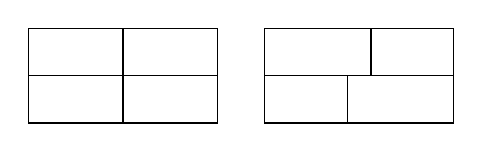
\begin{tikzpicture}[scale=0.3,line width=0.5pt] 
		%\draw[step=0.25cm,color=gray] (-3,-1) grid (3,1);
		
		% === Left rectangle
		\draw (-9, -2) rectangle (-1,+2);
		\draw (-9,  0) -- (-1,  0);
		\draw (-5, -2) -- (-5, +2);
		
		% === Right rectangle
		\draw (+1, -2) rectangle (+9,+2);
		\draw (+1,  0) -- (+9,  0);
		\draw (+4.5, -2) -- (+4.5,  0);
		\draw (+5.5,  0) -- (+5.5, +2);
		
		%\draw (0.60,0cm) node[above=1pt] {\small\em interior $c^\circ$};
		%\draw (-2.5,0cm) node[above=1pt] {\small\em exterior $c^-$};
		%\draw (-1.8,1.6cm) node[above=1pt] {\small\em boundary $\partial c$ = $C$};
		
		%\draw[dotted,line width=0.5pt] (-1.5, 1.65) -- (-0.75, 1.25);
		
		\end{tikzpicture}
		%[every node/.style={draw,fill=black,solid,inner sep=1pt,minimum size=4mm}]
		\end{center}
		\caption{A rectangular dissection (left) and its transformation into a $T$-plan (righr).}
		\label{dissectiontplan}
		\end{figure}
		
		If a rectangular space $R$ has been decomposed into $n$ rectangles $\{ r_1, \dots, r_n \}$,
		we say that we have a $T$-plan of order $n$. For example, Fig. \ref{dissectiontplan}
		(right) shows a $T$-plan of order $4$.
		
		Now let $h$, $v$, $s$ and $S$ be the following four partitioning operations: horizontal,
		vertical, left-spiral and right-spiral partitioning.
		$T*$-plans are those $T$-plans (i.e. rectangular dissections) which have been obtained by applying 
		exclusively these partitioning operations. (Therefore, $T* \subset T$.)
		
		\begin{figure}[h!]
		\centering
		\begin{tabular} {cccc}
		
			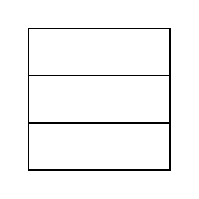
\begin{tikzpicture}[scale=0.3,line width=0.5pt] 
				\draw (0, 0) rectangle (6,6);
				\draw (0, 2) -- (6,2);
				\draw (0, 4) -- (6,4);
			\end{tikzpicture} &
		
			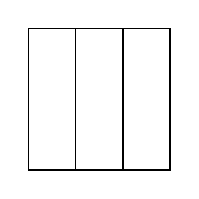
\begin{tikzpicture}[scale=0.3,line width=0.5pt] 
				\draw (0, 0) rectangle (6,6);
				\draw (2, 0) -- (2,6);
				\draw (4, 0) -- (4,6);
			\end{tikzpicture} &
		
			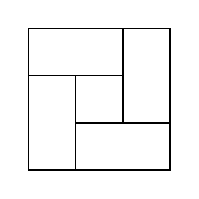
\begin{tikzpicture}[scale=0.3,line width=0.5pt] 
				\draw (0, 0) rectangle (6,6); % main rectangle
				\draw (0, 4) rectangle (4,6); % D1
				\draw (0, 0) rectangle (2,4); % D2
				\draw (2, 2) rectangle (4,4); % D3
				\draw (4, 2) rectangle (6,6); % D4
				\draw (2, 0) rectangle (6,2); % D5
			\end{tikzpicture} &
		
			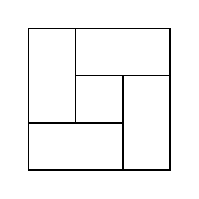
\begin{tikzpicture}[scale=0.3,line width=0.5pt] 
				\draw (0, 0) rectangle (6,6);
				\draw (0, 2) rectangle (2,6); % D1
				\draw (0, 0) rectangle (4,2); % D2
				\draw (2, 2) rectangle (4,4); % D3
				\draw (2, 4) rectangle (6,6); % D4
				\draw (4, 0) rectangle (6,4); % D5
			\end{tikzpicture} \\ \\
		
		$h$ & $v$ & $s$ & $S$ \\
		\end{tabular}
		\caption{Partitioning operations: 
		horizontal, vertical, left-spiral and right-spiral.}
		\label{operations}
		\end{figure}
		
		
		The author shows (giving a formal mathematical proof) that, 
		for a given $T*$-plan, 
		the subregion representation (which consists of nested regions, represented using trees) and 
		the wall
		representation (where each wall is written as an ordered pair of lists of the 
		basic regions adjacent to the wall) are equivalent in the sense that one can be obtained from the
		other in a unique fashion.
		
		An interesting paper, however, it's limited to rectangular
		spaces only. It is useful to know, though, that wall representation is equivalent to
		subregion representation. It would be interesting to see how one can generalize this work
		to regions of arbitrary shape.
		\end{quote}

\citeSK{woodbury2000erasure}
		\begin{quote}
		\small
		This exposition revolves around the notions of:\\
		- {\em typed feature structures}, a way to encode design states,\\
		- {\em subsumption}, a relation imposing ordering over such design states 
		  (i.e. typed feature structures) based on information specificity, and\\
		- {\em incremental $\pi$-resolution}, a way to generate new design states.
		\end{quote}

		
\citeSK{vander2001lessons}
		\begin{quote}
		\small
		Supported by their experiences with two GUI toolkits (List-based Garnet, and its 
		C++-based successor Amulet),
		the authors conclude that mark-sweep algorithms are superior to topological-sorting
		algorithms, within the context of one-way dataflow networks. Both toolkits 
		contain some innovative features: arbitrary Lisp and C++ code within constraints, 
		pointer variables
		(i.e. references), and support for cycles (i.e. the underlying parametric
		dependency graphs doesn't have to be acyclic). Pointer variables and
		conditionals (contained within constraints) lead to {\em dynamic dataflow graphs},
		graphs which can change structurally (through run-time additional or removal
		of edges) in the course of the constraint satisfaction process.
		
		\begin{figure}[htb]
		\begin{center}
		\includegraphics[width=0.8\textwidth]{figures/vander2001lessons.jpg}
		\caption{
		An example of dynamic dataflow graphs. 
		A, B, C and D represent rectangles.  
		Top: constraints can contain arbitrary code (e.g. C1 contains a conditional).
		Bottom: the graph has been changed dynamically by removing edge B.left $\rightarrow$ C3
		and adding new edge C.left $\rightarrow$ C3.
		\citeauthor{vander2001lessons}: 
		\citetitle{vander2001lessons} 
		\cite{vander2001lessons}.}
		\label{fig:vander2001lessons}
		\end{center}
		\end{figure}
		
		\end{quote}

		
%\citeSK{heisserman1993generating} 

\citeSK{kasik2005ten}
		\begin{quote}
		\small
	    Authors list ten CAD challenges in the following three areas:
	    \begin{enumerate}
	    
	    \item
	    {\it GEOMETRY:}
	        \begin{itemize}
	        \item Current methods for \emph{shape control} fail to preserve shape (person must
	        fix anomalies by hand),
	        \item There is no \emph{interoperability} between CAD, CAE, CFD etc. subsystems
	        (two major sources: FP arithmetic and tolerances)
	        \item \emph{Automatic design exploration} is not supported well (geometry does not morph 
	        continuously with parameters).
	        \end{itemize}
	        
	    \item        
	    {\it INTERACTION:}     
	        \begin{itemize}
	        \item Adding {\em simulation} earlier into the design process (this will enable consideration
	        of behavior, rather than just form; also, it will prevent some costly mistakes early in
	        the design process),
	        \item {\em Physical mobility} of a person and data (this can greatly increase agility
	        of thought; also, this brings increased opportunity for collaboration and increased
	        visibility of a particular activity),
	        \item {\em Reuse of components} (don't start from scratch; designers of assemblies, components;
	        devise components that scale because physical products don't scale with size).
	        \end{itemize}
	        
	    \item
	    {\it SCALE:}
	        \begin{itemize} 
	        \item {\em Understanding vast quantities of data} (integrated products must be examined from
	        a number of different views; product lifecycle management --- PLM),
	        \item Offering {\em different rendering/visualization types} for different professionals,
	        \item {\em Retrieving data} years later,
	        \item Fast and effective {\em collaboration over the net} (current 3D collaboration lacks immediacy and
	        extensive cues of a face-to-face session).
	        \end{itemize}
	        
	    \end{enumerate}
		\end{quote}

    
\citeSK{aish2005multi}
		\begin{quote}
		\small
		% SK: having just parametric modeling, although it's an advancement compared to conventional CAD,
		%     is not enough, because there is a very large number of possible relations between
		%     entities ('designs').
		%
		% SK: also, parametric CAD presupposes that we ALWAYS have to work with 3D representations
		%     (i.e. geometry in space, and its constraints) but this is too poor --- designed artifact
		%     can be represented in many different ways, not only 3D or parametric dependency graph.
		%     For example, as 2D diagrams, or 3D "clouds of points", or 3D "translucent spheres", and
		%     similar.
		%
		% SK: a thought: search engine which searches using different types of relations.
		%
		% SK: from the paper: "It turns out that the relationships that designers need to model
		%     their work comprise a set far too large and idiosyncratic to anticipate and provide
		%     as node types in a modelling environment". I basically agree with that; however,
		%     the problem is when the code-writing environment (i.e. API) doesn't expose enough
		%     functionality to code whatever relations I'd like to code.
		%     Also, what does it actually mean to "code a relation"? Isn't a relation supposed
		%     to be a set-membership, evaluated in some way (which way, and how many of ways
		%     are there)? For example, can GCScript be used to code Venn diagrams?
		%     SK idea: computing relations depends on the type of relations. For example,
		%     parametric dependencies should be computed in real-time as the user drags a 3D object.
		%
		% SK: idea: GC is too "heavy". An application must be quick, nimble, agile.
		%
		% SK: "In GC a node's independent variables can be either singletons or collections".
		%     What about references? For example, variable cs can be a reference to a coord. system.
		%
		% SK: node display algorithms must be user-modifiable! I.e. the user can specify whatever
		%     graphical representation he wants. In GC, display algorithms are predefined.
		%
		% SK: "The advantage of GC is that it helps me to think about what I am doing.
		%     The disadvantage is that it forces me to so think." --- Lars Hesselgren
		%     GC forces the user to think because the user has to specify relations whenever
		%     he creates/adds new element to the model.
		%     Instead, GC should adopt the approach from conventional CAD where the user just
		%     "puts" the component there, and the SYSTEM should help the user afterwards by either:
		%     1) not creating relations at all
		%     2) create default relations, using some AI module
		%     3) create "right" relations, well-adapted to the context, again using some AI
		% 
		% SK: Downside of GC is that the user has to manage FILES (e.g. .gtc files).
		%     The user should be relieved of this, and all changes/edits/modifications saved
		%     automatically, and presented nicely (through histories, etc.) so that the user
		%     can find everything easily afterwards.
		The article examines the implications of using parametric CAD tools (particulary
		in architectural design), and what are their main downsides and upsides.
		It also presents a concrete, novel (at the time) parametric CAD system, 
		{\em GenerativeComponents} (GC) by Bentley Systems Inc., as well as gives some
		anecdotal evidence on GC performance collected from individual users, and
		attendants of the SmartGeometry conference.
		\begin{figure}[htb]
		\begin{center}
		\includegraphics[width=0.5\textwidth]{figures/aish2005multi.jpg}
		\caption{
		GenerativeComponents by Bentley Systems Inc.  
		\citeauthor{aish2005multi}: 
		\citetitle{aish2005multi} 
		\cite{aish2005multi}.}
		\label{fig:aish2005multi}
		\end{center}
		\end{figure}				
		\end{quote}

% \citeSK{malak2009multi}  \\
% \citeSK{shai2009creative}  \\

%\afterpage{\clearpage}
%\nopagebreak
%\clearpage

\citeSK{attar2009physics}
		\begin{quote}
		The paper presents an {\em unified solver} for dynamics simulation,
		which dispenses with multiple solver types (e.g. rope solver, rigid body solver, \dots)
		usually needed to simulate
		different types of objects found in a given model.
		To achieve this, all objects in the model are represented by
		simplicial complexes (simplexes, or simplices). 
		The behavioural properties of the model are
		being defined through the following mechanism:
		1) vertices of the simplex are being computed as particles, and
		2) edges between vertices can assume three types of constraint:
		edge length, angle between two edges, and angle between two faces.
		
		\begin{figure}[htb]
		\begin{center}
		\includegraphics[width=0.4\textwidth]{figures/attar2009physics.jpg}
		\caption{
		Visualization of interacting forces.  
		\citeauthor{attar2009physics}: 
		\citetitle{attar2009physics} 
		\cite{attar2009physics}.}
		\label{fig:attar2009physics}
		\end{center}
		\end{figure}
		
		\end{quote}

%\citeSK{rutten2008grasshopper}
%\citeSK{payne2009grasshopper}
\citeSK{jennings2010phdthesis}
		\begin{quote}
		\small
		This thesis distills (from prior work) 
		ten principles for building ``good'' design-supporting systems,
		and makes a case for novel ways of evaluating human-computer interfaces based on 
		the concepts of {\em claims analysis}, {\em factual matrix}, and 
		{\em consilience} of factual matrix. (An explanation is more consilient if
		it explains more classes of fact.) To validate the principles
		according to these novel evaluation methods, 
		three system prototypes that follow (partially or fully) the proposed principles were built.
		%
		The first prototype, XDS, implements all ten principles to a degree, and provides
		experimental support for them. Users of XDS generate more alternatives,
		and improve on existing designs. XDS introduces two novel UI features:
		halo menus (Fig. \ref{fig:jennings2010phdthesis}), and consequence displays.
		%
		The second prototype, Strange Eons, operates in a different space (game space),
		thus enhancing the consilience of the factual matrix. It implements just some
		of the design principles, allowing for more controlled evaluation.
		%
		The third prototype, Treesta, shows that design principles have a degree of independence.
		
		\begin{figure}[htb]
		\begin{center}
		\includegraphics[width=0.2\textwidth]{figures/jennings2010phdthesis.jpg}
		\caption{
		When mouse cursor enters an object (gray rectangle), 
		a halo menu (hierarchical) appears.  
		\citeauthor{jennings2010phdthesis}: 
		\citetitle{jennings2010phdthesis} 
		\cite{jennings2010phdthesis}.}
		\label{fig:jennings2010phdthesis}
		\end{center}
		\end{figure}
		\end{quote}
		
%\citeSK{merrell2010computer} \\

\citeSKextended{woodbury2010elements}{Chapter 2: What is Parametric Modeling?}
		\begin{quote}
		\small
		This chapter of the book outlines essential features of parametric modeling 
		systems based on one-way data propagation constraints, including 
		nodes (including predecessor, successor nodes, source, sink and internal nodes), 
		links, dot notation, constraint expressions, node properties 
		(dependent and independent), parametric designs, graphs, directed graphs,
		directed acyclic graphs (DAGs), chains, three algorithm types (ordering,
		propagating, and displaying), topological ordering.
		
		\begin{figure}[htb]
			\centering
			\includegraphics[width=0.6\textwidth]{figures/woodbury2010elements.jpg}
			\caption{
			A simple parametric graph, and the corresponding code.  
			\citeauthor{woodbury2010elements}: 
			\citetitle{woodbury2010elements} 
			\cite{woodbury2010elements}.}
			\label{fig:woodbury2010elements}
		\end{figure}

		Objects can have multiple update algorithms, even as simple as points. 
		For example, when a point's location (unique in a physical world) 
		is updated in a Cartesian coordinate system,
		equivalent cylindrical coordinates ($\rho$, $\phi$ and $z$) are computed using
		Cartesian coordinates $x$, $y$ and $z$. And vice versa, if we see the point's
		location in cylindrical coordinate system.

		\begin{figure}[htb]
			\centering
			\includegraphics[width=0.9\textwidth]{figures/woodbury2010elements1.jpg}
			\caption{
			Two different update methods for a point object.
			\citeauthor{woodbury2010elements}: 
			\citetitle{woodbury2010elements} 
			\cite{woodbury2010elements}.}
			\label{fig:woodbury2010elements1}
		\end{figure}

						
		\end{quote}

\citeSK{bettig2011geometric}
		\begin{quote}
		\small
		This paper gives a survey of state of art in parametric operations and geometric
		constraint solving, whereby:\\
		- {\em parametric operations} denote operations such as {\em extrude}, which satisfy
		  some implied constraints, and\\
		- {\em geometric constraint solving} denotes operations which satisfy constraints
		  explicitly defined by the user, such as {\em repositioning}.\\
		The authors claims that the downsides of parametric operations include the need
		for the user to think ahead about how to manipulate the geometric features of objects,
		as well as to manage possible cycles in the underlying parametric graph. This
		is to be contrasted with geometric constraint solving, whereby objects (containing parameters)
		are being put into the scene first, and then these parameters are being linked
		through constraint links. This gap presents opportunities for new advancements.
		
		Within the paper, the concepts discussed include: 
		solver competence, constraint graphs, constraint graph structure analysis,
		approaches to geometric constraint solving 
		(graph based [constructive, DoF, propagation], logic-based, algebraic, symbolic, 
		theorem-prover based, numerical-methods based), deformations, dynamic geometry,
		evolutionary methods, three types of graph-constructive solvers (top-down, bottom-up,
		hybrid), graph decomposition, under- and over-constrained problems, variable-radius circles,
		valid parameter ranges, 3D constraints, open problems. 
		\begin{figure}[htb]
			\centering
			\includegraphics[width=0.6\textwidth]{figures/bettig2011geometric.jpg}
			\caption{
			Parametric operations vs. Geometric Constraint Solving.
			\citeauthor{bettig2011geometric}: 
			\citetitle{bettig2011geometric} 
			\cite{bettig2011geometric}.}
			\label{fig:bettig2011geometric}
		\end{figure}
		\end{quote}

\citeSK{gleicher2011visual}
		\begin{quote}
		\small
		Based on the analysis of existing approaches and systems for comparing objects,
		this paper demonstrates that ways to compare different designs can be classified into
		three categories: 
		{\em juxtaposition} (separate visualization of designs),
		{\em superposition} (designs visualized on top of each other), and
		{\em explicit encoding} (relations between designs are somehow encoded, for example
		the difference $X - Y$ of two different designs $X$ and $Y$).
		
		\begin{figure}[htb]
		\begin{center}
		\includegraphics[width=0.6\textwidth]{figures/gleicher2011visual.jpg}
		\caption{
		Categories of design comparison.  
		\citeauthor{gleicher2011visual}: 
		\citetitle{gleicher2011visual} 
		\cite{gleicher2011visual}.}
		\label{fig:gleicher2011visual}
		\end{center}
		\end{figure}
		
		\end{quote}

%\citeSK{bentley2011designplusplus} % Design++ \cite{bentley2011designplusplus},
%\citeSK{bentley2012gc}
%\citeSK{krygiel2010mastering} %Revit \cite{krygiel2010mastering}, 
%\citeSK{autodesk2012revit}



\subsection{Modeling, Representations} 

%\citeSK{bondy1976graph} \\
\citeSK{winston1987taxonomy}
		\begin{quote}
		\small
		The authors examine, from the standpoint of cognitive science, 
		the relations between {\em parts}, and the {\em wholes} which they make up ---
		the so-called {\em meronymic} relations. Meronymic relations are:\\
		- transitive (if $a$ is part of $b$, and $b$ is part of $c$, then $a$ is part of $c$),\\
		- irreflective ($a$ is not part of $a$), and\\
		- antisymmetric (if $a$ is part of $b$ then $b$ is not part of $a$).\\
		As such, meronymic relations express strict partial ordering, and 
		structure the semantic space (i.e. the space of all concepts) into a hierarchy.
		The question is, however, whether there are several (many?) different classes of
		relations expressing "parthood", or just one? To answer this question, the authors
		came up with the following taxonomy of of meroymic semantic relations,
		as expressed in everyday English:\\
		- component-integral (pedal-bike),\\
		- member-collection (ship-fleet),\\
		- portion-mass (slice-pie),\\
		- stuff-object (stell-car),\\
		- feature-activity (paying-shopping),\\
		- place-area (Everglades-Florida).
		\end{quote}
		
\citeSK{harel1988visual}
		\begin{quote}
		\small
		This paper discusses two well-known topo-visual formalisms (Venn diagrams, and
		graphs), and how to combine the two into a novel formalism, called {\em higraphs}.
		
		Venn diagrams have the capability to model {\em collections} of sets and 
		the following {\em structural} (i.e. set-theoretical) relationships between these sets:\\
		- {\em enclosure} (being-a-subset-of),\\
		- {\em exclusion} (being-disjoint-from), and\\
		- {\em intersection} (having-a-non-empty-intersection-with).
		
		On the other hand, mathematical graphs have the capability to model {\em connectedness}
		between vertices in a {\em single} set of elements $S$, with edges representing some
		(arbitrary) binary relation on elements in $S$. Thus, the information contained in
		graphs is {\em non-metric}: concepts like distance, shape and size have no meaning
		in graphs.
		
		Thus, graphs deal with a single set $S$; Venn diagrams deal with a 
		collection of sets $A_1, A_2, \dots, A_n$.
		%
		Graphs model relation(s) between elements of $S$ (using edges); Venn diagrams model set-theoretical 
		relationships ($\subset$, $\setminus$, $\cap$) between $A_1, A_2, \dots, A_n$.
		
		However, the author argues that in modern applications both capabilities are needed:
		large number of sets having set-theoretical relationships, {\em and} 
		some type of relation(s) (i.e. connectedness) among these sets. Furthermore,
		to prevent combinatorial explosion of Cartesian products, we often desire
		a representation capable of capturing the notion of Cartesian products in
		a compact way. The author thus presents a case for {\em higraphs}, which are
		built up in the following fashion: take Venn diagrams, augment them with the notion
		of "nesting curves", extend them to present Cartesian product, and 
		then connect them using edges or hyperedges.
		
		\begin{figure}[htb]
		\centering
		\includegraphics[width=0.5\textwidth]{figures/harel1988visual.jpg}
		\caption{
		A higraph, containing {\em atomic} sets B, C, E, \dots, {\em compound} sets
		A, P, R, T, \dots, and Cartesian products D = Y $\times$ Z, J = W $\times$ X.  
		\citeauthor{harel1988visual}: 
		\citetitle{harel1988visual} 
		\cite{harel1988visual}.}
		\label{fig:harel1988visual}
		\end{figure}
		
		\end{quote}

\citeSK{harada1995interactive}
		\begin{quote}
		\small
		Previous approaches to physics-based modeling were mostly limited to systems
		governed by continuous variables, without paying much attention to {\em structural}
		changes in the model (i.e. models which are governed by discrete variables as well). 
		This paper presents an approach to deal with this gap; basically, the approach
		suggests applying a discrete transformation (using a version of shape grammars) of the model 
		whenever an action in the model meets a hard geometric constraint.
		In other words, the authors suggest extending geometric/continuous simulations
		to allow the model to be subject to structural/discrete change, in response
		to some user action.
		
		\begin{figure}[htb]
		\centering
		\includegraphics[width=0.5\textwidth]{figures/harada1995interactive.jpg}
		\caption{
		Interactive geometric + structural change of the floorplan layout.
		\citeauthor{harada1995interactive}: 
		\citetitle{harada1995interactive} 
		\cite{harada1995interactive}.}
		\label{fig:harada1995interactive}
		\end{figure}
		
		\end{quote}

%\citeSK{shapiro2001solidmodeling}  \\

\citeSK{fritzson2002modelica}
		\begin{quote}
		\small
		This paper presents Modelica, a modeling language for building complex physical systems, 
		applicable to many different domains. Modelica features object-oriented design (with classes,
		and inheritance), equations which a acausal and thus do not prescribe flow directions,
		components, connectors, connections, and simulation capabilities (continuous and discrete).
		The language also features a number of packages, libraries, and a model editor (a graphical
		user interface for visually composing connection diagrams between components).
		
		\begin{figure}[htb]
		\centering
		\includegraphics[width=0.7\textwidth]{figures/fritzson2002modelica.jpg}
		\caption{
		Modelica: connecting two components through a connection (and associated connectors).
		\citeauthor{fritzson2002modelica}: 
		\citetitle{fritzson2002modelica} 
		\cite{fritzson2002modelica}.}
		\label{fig:fritzson2002modelica}
		\end{figure}
		
		\end{quote}

%\citeSK{botsch2006geometric}

\citeSK{muller2006procedural}
		\begin{quote}
		\small
		This paper introduces {\em CGA shape}, a special shape grammar (extension of set grammars) 
		devised for procedural modeling of buildings (i.e. shells thereof), 
		whose rules first generate an approximate volumetric model of a building,
		and then structure the facade and finally add surface details like windows and doors.
		In the process, the models are 1) created as a hierarchical structure, and
		2) the model is being annotated with semantic information. The authors
		illustrate the application of their approach in the following three cases:
		a simple (generic) building, office buildings, and single family homes.
		\begin{figure}[htb]
		\centering
		\includegraphics[width=0.7\textwidth]{figures/muller2006procedural.jpg}
		\caption{
		CGA shape example---procedural Pompeii model.
		\citeauthor{muller2006procedural}: 
		\citetitle{muller2006procedural} 
		\cite{muller2006procedural}.}
		\label{fig:muller2006procedural}
		\end{figure}
		
		\end{quote}

%\citeSK{botsch2008geometric} \\

\citeSK{whiting2009procedural}
		\begin{quote}
		\small
		This paper presents an approach to shape grammar-based 
		procedural modeling of (masonry) buildings with a twist:
		the generated buildings are automatically structurally sound, i.e. the buildings built according
		to these models would be able to carry their own weight.
		In other words, the authors
		present a method for generating masonry building geometry, based on physical constraints. 
		%
		Moreover, while in conventional 
		ways of designing a masonry building the analysis of structural validity is carried out 
		{\em post hoc} (i.e. after the building has been designed), the method suggested
		by authors in this paper automatically adjusts a set of free parameters {\em during the process}
		in order to obtain structurally sound masonry buildings. 
		%
		Thus there is no need
		to carry out a conventional structural analysis (which more often than not is relatively
		tedious) after the design has been completed. This way, even user with no experience
		in statics can design structurally sound masonry buildings.
		
		\begin{figure}[htb]
		\centering
		\includegraphics[width=0.99\textwidth]{figures/whiting2009procedural.jpg}
		\caption{
		Pipeline of the computation.
		\citeauthor{whiting2009procedural}: 
		\citetitle{whiting2009procedural} 
		\cite{whiting2009procedural}.}
		\label{fig:whiting2009procedural}
		\end{figure}
		
		\end{quote}

%\citeSK{friedenthal2011practical} %UML and SysML \cite{weilkiens2007systems}\cite{friedenthal2011practical},
%\citeSK{buildingsmart2012ifc}


\subsection{Creativity, Problem Solving} 
%\citeSK{simon1978information} \\
%\citeSK{newel1973knowledgelevel} \\

\citeSK{smith1998idea}
		\begin{quote}
		\small
		The author analyzes 172 different techniques for idea generation,
		and from this corpus distills 50 "idea-generation devices",
		classified into {\em strategies}, {\em tactics}, and {\em enablers}.
		\end{quote}

\citeSK{shneiderman2000creating}
		\begin{quote}
		\small
		Three perspectives on creativity:
		\begin{enumerate}
		
		\item \emph{Inspirationalist} --- emphasis on brain-storming, free association,
		lateral thinking and divergence. 
		% Corresponding software is based on free association 
		% using textual or graphical elements, visual techniques for depicting relationships,
		% loosely connected concept nodes to avoid a linear or hierarchical
		% structure, mind mapping. Paper and pencil, sketches.
		
		\item \emph{Structuralist} --- emphasis on more orderly approaches, like studying
		previous work and using methodical techniques to
		exhaustively explore possible solutions, then evaluate these solutions
		and refine them. 
		% Software: libraries, web sites,
		% "what-if" tools (spreadsheets, simulations, models, animations), flow
		% charts, decision trees, structured diagrams, step-by-step exploration, experimentation, backtracking.
		
		\item \emph{Situationalist} --- emphasis on social and intellectual context. 
		% Peer
		% reviews, curators, competitions, prize juries. Three
		% components: domain (e.g. mathematics), field (gatekeepers, curators),
		% and person.
		
		\end{enumerate}
		
		
		Three levels of creativity:
		
		\begin{enumerate}
		
		\item Great breakthroughs and paradigm-shifting
		innovations. E.g. Einstein's relativity theory, Watson
		and Crick's DNA discovery, Stravinsky's "Rite of Spring"
		
		\item Evolutionary creativity (the focus of this
		article) - useful evolutionary contributions that refine
		and apply existing paradigms. Normal science, doctors' diagnoses,
		lawyers' briefs, photo editors' stories.
		
		\item Impromptu/personal creativity. Lively
		conversation, attentive parenting.
		
		\end{enumerate}
		
		Four-phase genex framework (with eight primary activities):
		
		\begin{enumerate}
		
		\item \emph{Collect}
			\begin{itemize}
			\item Searching and browsing digital libraries
			\item Visualizing data and processes
			\end{itemize}
		       
		\item \emph{Relate}
			\begin{itemize}
			\item Consulting with peers and mentors
			\end{itemize}
		       
		\item \emph{Create}
			\begin{itemize}
			\item Thinking by free associations
			\item Exploring solutions - what-if tools
			\item Composing artifacts and performances
			\item Reviewing and replaying session histories
			\end{itemize}
		       
		\item \emph{Donate}
			\begin{itemize}
			\item Disseminating results
			\end{itemize}
		\end{enumerate}
		
		       
		% All objects in the genex framework (like e.g. lists, or diagrams) should be
		% easily shared with others, annotatable, linkable and searchable.
		\end{quote}

% \citeSK{nishino20013d}	
% 		\begin{quote}
% 		\small
% 		
% 		\end{quote}

%\citeSK{takagi2001interactive}	
		
\citeSK{warr2005understanding}
		\begin{quote}
		\small
		Based on the analysis of existing models of creativity, the authors suggest
		an unified model named {\em Generic Creative Process Model}; see Fig. \ref{fig:warr2005understanding}.
		Their model consist of three phases: Problem Preparation, Idea Generation, and Idea Evaluation.
		\begin{figure}[htb]
		\begin{center}
		\includegraphics[width=2.5in]{figures/warr2005understanding.jpg}
		\caption{Generic Creative Process Model according to Warr and O'Neill \cite{warr2005understanding}.}
		\label{fig:warr2005understanding}
		\end{center}
		\end{figure}				
		\end{quote}		

\citeSK{shneiderman2006creativity}
		\begin{quote}
		\small
		The paper argues that what was Galileo's telescope, Thomas Jefferson's pantograph, 
		and similar devices in the past,
		software tools have become today---they will support creativity and thus enable new discoveries.
		Three key components of creativity: {\em domain} (e.g. mathematics),
		{\em field} (gatekeepers), and {\em individual}, so creativity is after all a social process
		(because it's the gatekeepers who deem a work to be "creative").
		The goals of the workshop were:
		1) to call for greater convergence of disciplines that are in any way related to creativity,
		2) to promote new research methods, and
		3) increase the ambitiousness and scope of creativity-related research programs.
		The authors propose a set of principles to be used in building tools that support creativity: 
		1) support exploration,
		2) low threshold (easy entry for novices), high ceiling (for experts), and wide walls (wide range
		of possible explorations), 
		3) support many paths and many styles, 
		4) support collaboration, 
		5) support open exchange, 
		6) make it as simple as possible---and maybe even simpler,
		7) choose black boxes carefully,
		8) invent things that you want to use yourself,
		9) balance user suggestions with observation and participatory process,
		10) iterate, iterate---then iterate again,
		11) design for designers,
		12) evaluate your tools.
		The report also suggest directions for further research: 
		1) evolve existing and develop new theories of creativity,
		2) identify the fundamental role of creativity in all disciplines,
		3) propose new tools that facilitate and enhance creativity,
		4) design socio-technological environments for creativity,
		5) formulate systematic foundations for distribution of creativity tools,
		6) develop new assessment methods, and
		7) emphasize education and learning.
		\end{quote}		

% \citeSK{kules2005supporting}
% 		\begin{quote}
% 		\small
% 		TBD
% 		\end{quote}
		
				
\citeSK{ritchey2006problem}
		\begin{quote}
		\small
		The paper describes General Morphological Analysis (GMA), a problem-structuring method
		which avoids committing itself to quantitative cause-and-effect constraints, 
		i.e. is capable to express non-quantifiable constraints prevalent in ill-defined problems.
		In other words, GMA is not based on building graphs of causal relations and/or
		hierarchical structures, but on parameter dimensions constrained by logical relations 
		(see Fig. \ref{fig:ritchey2006problem} for an example).
		By indicating pair-wise inconsistency between dimensions, the method effectively
		eliminates entire (sub)sets of unfeasible configurations, 
		thus greatly simplifying the initial problem.
		\begin{figure}[htb]
		\begin{center}
		\includegraphics[width=4in]{figures/ritchey2006problem.jpg}
		\caption{An example for General Morphological Analysis (GMA),
		see Ritchey \cite{ritchey2006problem}. The sample problem contains 6 parameters and
		N=576 possible configurations (4*4*3*3*2*2), of which one valid configuration (i.e. choice of
		parameters) is highlighted. By indicating inconsistent relationships, N can be significantly
		reduced, thus simplifying the initial problem.} 
		\label{fig:ritchey2006problem}
		\end{center}
		\end{figure}						
		\end{quote}

\citeSK{shneiderman2007creativity}
		\begin{quote}
		\small
		There is a recent shift underway, from productivity support tools, to creativity support tools.
		These tools cannot be evaluated using conventional measures like time per task,
		cost per transaction, and similar, thus new evaluation methods are needed.
		Next, the author suggests a way forward in research related to creativity support tools, 
		by first focusing on developing tools
		that support 
		1) discovery in the sciences, 
		2) exploration in design, 
		3) innovation in engineering, and 
		4) imagination in the arts.
		To define creative processes, the author then goes on to first list three intersecting
		schools on creativity (structuralists, inspirationalists, and situationalists),
		then three Csikszentmihalyi's definitions (domain, field, individual),
		and three important mindset changes needed (developers, product managers, and researchers).
		The author proposes the following design principles for creativity support tools:
		1) support exploratory search,
		2) enable collaboration,
		3) provide rich history-keeping, and
		4) design with low thresholds, high ceilings, and wide walls.
		The author then suggest an assortment of techniques which could be applied in
		evaluting creativity support tools.
		\end{quote}

% \citeSK{howard2008describing}
% 		\begin{quote}
% 		\small
% 		Gives an account of creativity from the cognitive science standpoint, and in the context
% 		of engineering design.
% 		\end{quote}


% \subsection{Requirements and Goal Engineering} 
% \citeSK{yu1997towards}  \\
% \citeSK{van2001goal} \\
% \citeSK{erhan2003interactive} \\ 
% \citeSK{sommerville2005integrated} \\ 
% \citeSK{chung2009nonfunctional}
% 
% 
% \subsection{Prototype-Based Computing} 
% \citeSK{borning1986classes} \\ 
% \citeSK{taivalsaari1997classes} 


\subsection{Histories, Versioning, Undo/Redo} 

\citeSK{kurlander1990visual}
		\begin{quote}
		\small
		This paper reports an approach to visualizing and working with histories of drawing operations,
		through a prototype image editor named Chimera.
		The two most important concepts presented are:\\
		- pictorial series of prologue-epilogue pairs (thumbnails) giving some insight into
		what changed in an affected part of the image, and\\
		- using these series as a way to implement redo and undo.
		\begin{figure}[htb]
		\centering
		\includegraphics[width=0.99\textwidth]{figures/kurlander1990visual.jpg}
		\caption{
		The final image drawn (left), and the history of drawing operations (shown as
		a sequence of prologue-epilogue pairs into relevant parts of the image)(right).
		Each of these prologue-epilogue pairs can be expanded further, into even finer
		sequences of prologue-epilogue pairs.
		\citeauthor{kurlander1990visual}: 
		\citetitle{kurlander1990visual} 
		\cite{kurlander1990visual}.}
		\label{fig:kurlander1990visual}
		\end{figure}
				
		\end{quote}

		

% \citeSK{sun1998operational}
% 		\begin{quote}
% 		\small
% 		TBD
		
% 		\begin{figure}[htb]
% 		\centering
% 		\includegraphics[width=0.99\textwidth]{figures/sun1998operational.jpg}
% 		\caption{
% 		TBD.
% 		\citeauthor{sun1998operational}: 
% 		\citetitle{sun1998operational} 
% 		\cite{sun1998operational}.}
% 		\label{fig:sun1998operational}
% 		\end{figure}
% 				
% 		\end{quote}
						

% \citeSK{sun2000undo}
% 		\begin{quote}
% 		\small
% 		TBD
		
% 		\begin{figure}[htb]
% 		\centering
% 		\includegraphics[width=0.99\textwidth]{figures/sun2000undo.jpg}
% 		\caption{
% 		TBD.
% 		\citeauthor{sun2000undo}: 
% 		\citetitle{sun2000undo} 
% 		\cite{sun2000undo}.}
% 		\label{fig:sun2000undo}
% 		\end{figure}
% 				
% 		\end{quote}
				
				
% \citeSK{edwards2000temporal}
% 		\begin{quote}
% 		\small
% 		sdkfjsk
		
% 		\begin{figure}[htb]
% 		\centering
% 		\includegraphics[width=0.99\textwidth]{figures/edwards2000temporal.jpg}
% 		\caption{
% 		TBD.
% 		\citeauthor{edwards2000temporal}: 
% 		\citetitle{edwards2000temporal} 
% 		\cite{edwards2000temporal}.}
% 		\label{fig:edwards2000temporal}
% 		\end{figure}
% 				
% 		\end{quote}

\citeSK{klemmer2002web}
		\begin{quote}
		\small
		This article presents an approach to collecting and navigating alternatives in 
		web design. The device used was Designers' Post,
		a wall-sized tangible interface for collaborative design. % (Fig. \ref{fig:klemmer2002web}).
		The authors present a way to interact with histories, without forcing the user
		to cope with a cognitively-demanding complete derivation tree, through the use of 
		the so-called {\em stub-branching history presentation} (Fig. \ref{fig:klemmer2002web2}).
		In the simple qualitative evaluation study, the participants (professional web designers)
		suggested features for simultaneous comparison and merging of history states.
		\begin{figure}[htb]
		\begin{center}
		\includegraphics[width=0.7\textwidth]{figures/klemmer2002web2.jpg}
		\caption{
		Stub-branching history presentation.  
		\citeauthor{klemmer2002web}: 
		\citetitle{klemmer2002web} 
		\cite{klemmer2002web}.}
		\label{fig:klemmer2002web2}
		\end{center}
		\end{figure}
 		\end{quote}
		
% 		\begin{figure}[h!]%[htb]
% 		\begin{center}
% 		\includegraphics[width=0.6\textwidth]{figures/klemmer2002web.jpg}
% 		\includegraphics[width=0.99\textwidth]{figures/klemmer2002web1.jpg}
% 		\caption{
% 		Designers' Outpost. The bottom contains the main timeline; each thumbnail
% 		represents the contents of the board at the time of capture. Elements
% 		that were changed in a design (compared to a previous design), are highlighted.  
% 		\citeauthor{klemmer2002web}: 
% 		\citetitle{klemmer2002web} 
% 		\cite{klemmer2002web}.}
% 		\label{fig:klemmer2002web}
% 		\end{center}
% 		\end{figure}
% 		\end{quote}
		

% \citeSK{cass2006empirical}
% 		\begin{quote}
% 		\small
% 		TBD
		
% 		\begin{figure}[htb]
% 		\centering
% 		\includegraphics[width=0.99\textwidth]{figures/cass2006empirical.jpg}
% 		\caption{
% 		TBD.
% 		\citeauthor{cass2006empirical}: 
% 		\citetitle{cass2006empirical} 
% 		\cite{cass2006empirical}.}
% 		\label{fig:cass2006empirical}
% 		\end{figure}
% 				
% 		\end{quote}
				
%\citeSK{torvalds2006git} \\

\citeSK{heer2008graphical}
		\begin{quote}
		\small
		The authors present the design and implementation of graphical history tools based
		on Tableau, a contemporary multi-dimensional database visualization system.
		They first give a short survey on how to store and structure history data (states,
		actions, or both), how to visualize history data (linear, branching, \dots),
		and how to interact with history (navigation, editing, search, and export).
		They then go on their approach in Tableau:\\
		- they adopted a hybrid state/action history model,\\
		- states are recorded as VizQL statements,\\
		- each action is classified into one of the following five categories:
		  shelf (add, remove, replace), data (bin, derive field), analysis (filter, sort),
		  worksheet (add, delete, duplicate), and formatting (resize, style) commands.\\
		- all basic history items can be grouped into composites,\\
		- when user visits a past state and performs an action, a new analysis branch is
		  added to the model,\\
		- support for merged histories.\\
		The history model in Tableau is visualized using a sequential, comic-strip display.
		Additional features include analyzing individual usage (based on behaviour graphs),
		and aggregate usage. Findings based on usage data:\\
		- undo was 12 times more common than redo,\\
		- formatting accounts for 24\% of all actions.  
		\begin{figure}[htb]
		\begin{center}
		\includegraphics[width=0.5\textwidth]{figures/heer2008graphical.jpg}
		\caption{
		An instance of history (top), and its visualization (bottom).  
		\citeauthor{heer2008graphical}: 
		\citetitle{heer2008graphical} 
		\cite{heer2008graphical}.}
		\label{fig:heer2008graphical}
		\end{center}
		\end{figure}

		\end{quote}


% \citeSK{su2009interactive}
% 		\begin{quote}
% 		\small
% 		TBD
		
% 		\begin{figure}[htb]
% 		\centering
% 		\includegraphics[width=0.99\textwidth]{figures/su2009interactive.jpg}
% 		\caption{
% 		TBD.
% 		\citeauthor{su2009interactive}: 
% 		\citetitle{su2009interactive} 
% 		\cite{su2009interactive}.}
% 		\label{fig:su2009interactive}
% 		\end{figure}
				
% 		\end{quote}
		


% \citeSK{sarvghad2009history}
% 		\begin{quote}
% 		\small
% 		TBD
		
% 		\begin{figure}[htb]
% 		\centering
% 		\includegraphics[width=0.99\textwidth]{figures/sarvghad2009history.jpg}
% 		\caption{
% 		TBD.
% 		\citeauthor{sarvghad2009history}: 
% 		\citetitle{sarvghad2009history} 
% 		\cite{sarvghad2009history}.}
% 		\label{fig:sarvghad2009history}
% 		\end{figure}
				
% 		\end{quote}
				
% \citeSK{chacon2009pro} \\
% \citeSK{altmanninger2009survey} \\ 
% \citeSK{ruparelia2010history}\\


% \citeSK{grossman2010chronicle}
% 		\begin{quote}
% 		\small
% 		TBD
% 		
% % 		\begin{figure}[htb]
% % 		\centering
% % 		\includegraphics[width=0.99\textwidth]{figures/grossman2010chronicle.jpg}
% % 		\caption{
% % 		TBD.
% % 		\citeauthor{grossman2010chronicle}: 
% % 		\citetitle{grossman2010chronicle} 
% % 		\cite{grossman2010chronicle}.}
% % 		\label{fig:grossman2010chronicle}
% % 		\end{figure}
% 				
% 		\end{quote}


% \citeSK{lutteroth2011rewriting}
% 		\begin{quote}
% 		\small
% 		TBD
% 		
% % 		\begin{figure}[htb]
% % 		\centering
% % 		\includegraphics[width=0.99\textwidth]{figures/lutteroth2011rewriting.jpg}
% % 		\caption{
% % 		TBD.
% % 		\citeauthor{lutteroth2011rewriting}: 
% % 		\citetitle{lutteroth2011rewriting} 
% % 		\cite{lutteroth2011rewriting}.}
% % 		\label{fig:lutteroth2011rewriting}
% % 		\end{figure}
% 				
% 		\end{quote}

% \citeSK{koc2011survey} \\ 
% \citeSK{raymond2012understanding}
%\citeSK{pilato2008version} %Subversion \cite{pilato2008version}\cite{berlin2006practical},


% \subsection{General Computing and Miscellaneous} 
% %\citeSK{winston1987taxonomy} 
% %\citeSK{brin1998anatomy} 
% %\citeSK{thomas2006visual} 

% \citeSK{graham2010survey} 


	
